\documentclass{article}

\usepackage{graphicx}
\usepackage{lmodern}
\usepackage{enumitem}

\begin{document}
	\begin{titlepage}
		\fontfamily{pbk}\selectfont
		\hbox{			
			\rule{1pt}{\textheight}
			\hspace*{0.05\textwidth}
			\parbox[b]{\textwidth}{
				\Large Project Tender\\[1cm]
					
				\Huge Project: Harvest\\
				\huge Client: Subtrop\\[1.5cm]					
					
				{\huge Team: HTTP\textunderscore418}
				
				\begin{itemize}[label={}, leftmargin=0pt, noitemsep]
					\Large						
					\item Christiaan Saaiman, 12059138
					\item Michael Loosen, 14017254
					\item Elizabeth Bode, 14310156
					\item LC Meyers, 14024633
				\end{itemize}
				\vspace{0.5cm}
					
				{\large Department of Computer Science, University of Pretoria\\[0.2cm]}

				\Large\today\\[0.3cm]				
									
				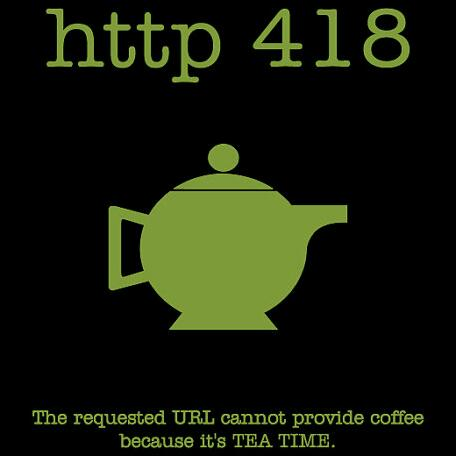
\includegraphics[scale=0.3]{../teamPic.jpg}					
			}								
		}
	\end{titlepage}
	\newpage
	\section{The Team}
	\subsection{LC Meyers}
	\begin{figure}[h]
		\centering
		
\includegraphics[height=0.3\textheight]{../charl.jpg}
	\end{figure}
	\begin{itemize}
		\item \textbf{Full name:} Lodewyk Charles Meyers
		\item \textbf{My interests:}
			\subitem Gaming
			\subitem Computers
			\subitem Music
			\subitem User experience design
			\subitem Website design
			\subitem Anything new related to technology
		\item \textbf{My technical skills:}
			\subitem Web development skills
			\subitem Database design
			\subitem Java
			\subitem C\#
		\item \textbf{Past experience that might help:}
			\subitem I have collaborated in an Android app made using PhoneGap
		\item \textbf{Non-technical strenghts:}
			\subitem I have a high amount of patience
			\subitem Hardworking
			\subitem Eager to learn new things
			\subitem Enjoy trying to solve complex problems
		\item \textbf{What makes me want to do this project?} Doing  this project sounds like it can be fun. It sounds like I might learn something new in the Subtropical industry. It will also be interesting to see how the service is being realised to help the farmers determine better yields. Finally it would be nice to learn how to create an app that uses GPS and other technologies needed for this project.
	\end{itemize}
	
	\section{Project excecution}
		\subsection{Technologies we will use for the project:}
			\begin{itemize}
				\item For the front end we will use Cordova along with Ionic as these technologies makes creating hybrid mobile apps easier. This means minimal code will need to be changed to make the app compatible with both Android and iOS. Since this front end is in essance a website and therefore will go nicely with a clien/server architecture.
				\item For the backend we will use PHP along with the Laravel framework for PHP. PHP is a very popular web language and is the langauge that most hired web servers run on. Laravel is a new and growing framework for PHP that makes abstracting the database and making RESTful services very easy.
				\item For persistence we will use MySQL. It is a very popular Relational Databasa Management System that is also iscluded in a lot of hired web servers. Making setup very easy. We also do not anticipate that too much data will be persisted for MySQL to become unreliable.
				\item If no web server is provided we can subscribe to any webhosting service that is very cheap to subscribe to a shared Linux server.
			\end{itemize}
\end{document}